\title{THE DILOGARITHM FUNCTION IN GEOMETRY AND NUMBER THEORY$^{1}$}
\footnotetext[1]{This paper is a revised version of a lecture given in Bonn on the occasion of F. Hirzebruch's 60th birthday, (October 1987) and has also appeared under the title ``The remarkable dilogarithm'' in the Journal of Mathematical and Physical Sciences, 22(1988).}
\markright{The Dilogarithm Function in Geometry and Number Theory}


\author{By~ D. Zagier}
\markboth{D. Zagier}{The Dilogarithm Function in Geometry and Number Theory}

\date{}
\maketitle

\setcounter{pageoriginal}{230}
\textsc{The\pageoriginale dilograrithm Function} is the function defined by the power series
$$
\Li_{2}(z)=\sum\limits_{n=1}^{\infty} \frac{z^{n}}{n^{2}}\quad\text{for~ } |z|<1.
$$

The definition and the name, of course, come from the analogy with the Taylor series of the ordinary logarithm around 1,
$$
-\log (1-z)=\sum\limits^{\infty}_{n=1}\frac{z^{n}}{n}\quad\text{for~ } |z|<1,
$$
which leads similarly to the definition of the {\em polylogarithm}
$$
\Li_{m}(z)=\sum\limits^{\infty}_{n=1}\frac{z^{n}}{n^{m}}\quad\text{for~ } |z|<1, \ m=1,2,\ldots
$$
The relation
$$
\frac{d}{dz}\Li_{m}(z)=\frac{1}{z}\Li_{m-1}(z)\quad (m\geq 2)
$$
is obvious and leads by induction to the extension of the domain of definition of $\Li_{m}$ to the cut plane $\mathbb{C}-(1,\infty)$; in particular, the analytic continuation of the dilogarithm is given by
$$
\Li_{1}(z)=-\int\limits^{z}_{0}\log (1-u)\frac{du}{u}\quad\text{for~ } z\in \mathbb{C}-(1,\infty).
$$
\begin{figure}[H]
\centering
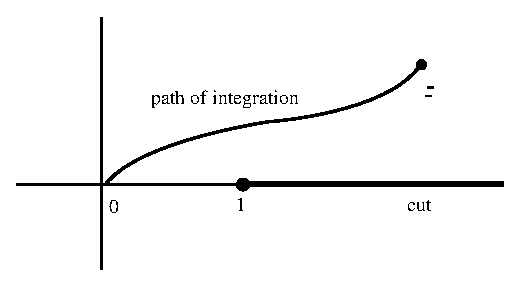
\includegraphics[scale=.9]{figures/fig1.eps}
\end{figure}

Thus\pageoriginale the dilogarithm is one of the simplest non-elementary functions one can imagine. It is also one of the strangest. It occurs not quite often enough, and in not quite an important enough way, to be included in the Valhalla of the great transcendental functions --- the gamma function, Bessel and Legendre functions, hypergeometric series, or Riemann's zeta function. And yet it occurs too often, and in far too varied contexts, to be dismissed as a mere curiosity. First defined by Euler, it has been studied by some of the great mathematicians of the past --- Abel, Lobachevsky, Kummer, and Ramanujan, to name just a few --- and there is a whole book devoted to it \cite{art15-key4}. Almost all of its appearances in mathematics, and almost all the formulas relating to it, have something of the fantastical in them, as if this function alone among all others possessed a sense of humor. In this paper we wish to discuss some of these appearances and some of these formulas, to give at least an idea of this remarkable and too little-known function.

\section{Special values}\label{art15-sec1}
Let us start with the question of special values. Most functions have either on exactly computable special values (Bessel functions, for instance) or else a countable, easily describable set of them; thus, for the gamma function
$$
\Gamma(n)=(n-1)!, \ \Gamma\left(n+\dfrac{1}{2}\right)=\dfrac{(2n)!}{2^{n}n!}\sqrt{\pi},
$$
and for the Riemann zeta function
\begin{align*}
& \zeta(2) =\dfrac{\pi^{2}}{6},\quad \zeta(4)=\dfrac{\pi^{4}}{90},\quad \zeta(6)=\dfrac{\pi^{6}}{945},\ldots,\\
& \zeta(0)=-\dfrac{1}{2},\quad \zeta(-2)=0,\quad \zeta(-4)=0,\ldots,\\
& \zeta(-1)=-\dfrac{1}{12},\quad \zeta(-3)=\dfrac{1}{120},\quad \zeta(-5)=-\dfrac{1}{252},\ldots.
\end{align*}

Now so the dilogarithm. As far as anyone knows, there are exactly eight values of $z$ for which $z$ and $\Li_{2}(z)$ can both be given in closed form :
\begin{align*}
\Li_{2}(0) &=0\\
\Li_{2}(1) &= \dfrac{\pi^{2}}{6},\\
\Li_{2}(-1) &= -\dfrac{\pi^{2}}{12},\\
\Li_{2}\left(\dfrac{1}{2}\right) &= \frac{\pi^{2}}{12}-\dfrac{1}{2}\log^{2}(2),\\
\Li_{2}\left(\dfrac{3-\sqrt{5}}{2}\right) &\dfrac{\pi^{2}}{15}-\log^{2}\left(\dfrac{1+\sqrt{5}}{2}\right),\\
\Li_{2}\left(\dfrac{-1+\sqrt{5}}{2}\right) &=\dfrac{\pi^{2}}{10}-\log^{2}\left(\dfrac{1+\sqrt{5}}{2}\right),\\
\Li_{2}\left(\dfrac{1-\sqrt{5}}{2}\right) &=-\dfrac{\pi^{2}}{15}+\dfrac{1}{2}\log^{2}\left(\dfrac{1+\sqrt{5}}{2}\right),\\
\Li_{2}\left(\dfrac{-1-\sqrt{5}}{2}\right) &=-\dfrac{\pi^{2}}{10}+\dfrac{1}{2}\log^{2}\left(\dfrac{1+\sqrt{5}}{2}\right).
\end{align*}\pageoriginale

Let me describe a recent experience where these special values figures, and which admirably illustrates what I said about the bizarreness of the occurrences of the dilogarithm in mathematics. From Bruce Berndt via Henri Cohen I learned of a still unproved assertion in the Notebooks of Srinivasa Ramanujan (Vol. 2, p. 289, formula (4)) : Ramanujan says that, for $q$ and $x$ between $0$ and $1$,
$$
\cfrac{q}{x+\cfrac{q^{4}}{x+\cfrac{q^{8}}{x+\cfrac{q^{12}}{x+_{\displaystyle\ddots}}}}} = 1- \cfrac{q^{x}}{1+\cfrac{q^{2}}{1-\cfrac{q^{3}x}{1+\cfrac{q^{4}}{1-\cfrac{q^{5}x}{1+_{\displaystyle\ddots}}}}}}
$$
``very nearly.'' He does not explain what this means, but a little experimentation shows that what is meant is that the two expressions are numerically very close when $q$ is near $1$; thus for $q=0.9$ and $x=0.5$ one has
\begin{center}
LHS = 0.7767340194\ldots,\qquad RHS = 0.7767340180....
\end{center}\pageoriginale

A graphical illustration of this is also shown.
\begin{figure}[H]
\centering
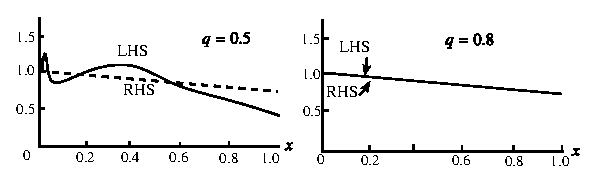
\includegraphics[scale=1.1]{figures/fig2.eps}
\end{figure}

The quantitative interpretation turned out as follows \cite{art15-key9} : The difference between the left and right sides of Ramanujan's equation is $O\dfrac{\pi^{2}/5}{(e^{\log}q)}$ for $x=1$, $q\to 1$ (the proof of this used the identities
$$
1+\cfrac{1}{1+\cfrac{q}{1+\cfrac{q^{2}}{1+\cfrac{q^{3}}{1+\qquad }{}}}}=\prod\limits^{\infty}_{n=1}(1-q^{n})^{\left(\frac{n}{5}\right)}=\dfrac{\Sigma(-1)^{r}q^{(5r^{2}+3r)/2}}{\Sigma(-1)^{r}q^{(5r^{2}+r)/2}}
$$
which are consequences of the Rogers-Ramanujan identities and are surely among the most beautiful formulas in mathematics). For $x\to 0$ and $q\to 1$ the difference is question is $O(e^{(\pi^{2}/4)/\log q})$, and for $0<x<1$ and $q\to 1$ it is $O(e^{c(x)/\log q})$ where $c'(x)=0(1/x)$ arcsinh $(x/2)=-\frac{1}{x}\log (\sqrt{1+x^{2}/4}+x/2)$. For these three formulas to be compatible, one needs
$$
\int\limits^{1}_{0}\frac{1}{x}\log(\sqrt{1+x^{2}/4}+x/2)dx=c(0)=c(1)=\dfrac{\pi^{2}}{4}-\dfrac{\pi^{2}}{5}=\dfrac{\pi^{2}}{20}.
$$

Using integration by parts and formula A.3.1 (6) of \cite{art15-eq1} one finds
\begin{align*}
& \int\frac{1}{x}\log (\sqrt{1+x^{2}/4}+x/2)dx=-\dfrac{1}{2}\Li_{2}\left((\sqrt{1+x^{2}/4}-x/2)^{2}\right)-\\
& -\frac{1}{2}\log^{2}\left(\sqrt{1+x^{2}/4}+x/2\right)+(\log x)\log\left(\sqrt{1+x^{2}/4}+x/2\right)+C,
\end{align*}\pageoriginale
so
\begin{align*}
& \int\limits^{1}_{0}\frac{1}{x}\log \left(\sqrt{1+x^{2}/4}+x/2\right)dx\\
&=\frac{1}{2}\Li_{2}(1)-\frac{1}{2}\left(\Li_{2}\left(\frac{3-\sqrt{5}}{2}\right)+\log^{2}\left(\frac{1+\sqrt{5}}{2}\right)\right)\\
&=\frac{\pi^{2}}{12}-\frac{\pi^{2}}{30}=\frac{\pi^{2}}{20}!
\end{align*}

\section{Functional equations}\label{art15-sec2}
In contrast to the paucity of special values, the dilogarithm function satisfies a plethora of functional equations. To begin with, there are the two reflection properties
\begin{align*}
& \Li_{2}(1/z)=-\Li_{2}(z)-(\pi^{2}/6)-(1/2)\log^{2}(-z)\\
& \Li_{2}(1-z)=-\Li_{2}(z)+(\pi^{2}/6)-\log(z)\log (1-z).
\end{align*}
Together they say that the six functions
$$
\Li_{2}(z), \Li_{2}\left(\dfrac{1}{1-z}\right), \Li_{2}\left(\dfrac{z-1}{z}\right), -\Li_{2}\left(\dfrac{1}{z}\right), -\Li_{2}(1-z), -\Li_{2}\left(\dfrac{z}{z-1}\right)
$$
are equal modulo elementary functions. Then there is the duplication formula
$$
\Li_{2}(z^{2}), \Li_{2}\left(\dfrac{1}{1-z}\right),\Li_{2}\left(\dfrac{z-1}{z}\right),-\Li_{2}\left(\dfrac{1}{z}\right),-\Li_{2}(1-z),-\Li_{2}\left(\dfrac{z}{z-1}\right)
$$
are equal modulo elementary functions. Then there is the duplication formula
$$
\Li_{2}(z^{2})=2(\Li_{2}(z)+\Li_{2}(-z))
$$
and more generally the ``distribution property''
$$
\Li_{2}(x)=n\sum\limits_{z^{n}=x}\Li_{2}(z)\quad (n=1,2,3,\ldots).
$$
Next, there is the two-variable, five-term relation
\begin{gather*}
\Li_{2}(x)+\Li_{2}(y)+\Li_{2}\left(\dfrac{1-x}{1-xy}\right)+\Li_{2}(1-xy)+\Li_{2}\left(\dfrac{1-y}{1-xy}\right)\\
=\frac{\pi^{2}}{2}-\log(x)\log(1-x)-\log(y)\log(1-y)+\log\left(\dfrac{1-x}{1-xy}\right)\log\left(\dfrac{1-y}{1-xy}\right)
\end{gather*}
which (in this or one of the many equivalent forms obtained by applying the symmetry properties given above) was discovered and rediscovered by Spence (1809). Abel (1827), Hill (1828), Kummer (1840), Schaeffer (1846),\pageoriginale and doubtless others. (Despite appearances, this relation is symmetric in the five arguments : if these are numbered cyclically as $z_{n}$ with $n\in \mathbb{Z}/5\mathbb{Z}$, then $1-z_{n}=\dfrac{z_{n-1}}{1-z_{n-1}}\dfrac{z_{n+1}}{1-z_{n+1}}=z_{n-2}z_{n+2}.$) There is also the six-term relation
\begin{align*}
\frac{1}{x}+\frac{1}{y}+\frac{1}{z} &= 1\Rightarrow \Li_{2}(x)+\Li_{2}(y)+\Li_{2}(z)\\
&= \frac{1}{2}\left[\Li_{2}\left(-\dfrac{xy}{z}\right)+\Li_{2}\left(-\dfrac{yz}{x}\right)+\Li_{2}\left(-\dfrac{zx}{y}\right)\right]
\end{align*}
discovered by Kummer (1840) and Newman (1892). Finally, there is the strange many-variable equation
\begin{equation}
\Li_{2}(z)=\sum\limits_{\substack{f(x)=z\\ f(z)=1}}\Li_{2}\left(\dfrac{x}{a}\right)+C(f),\label{art15-eq1}
\end{equation}
where $f(x)$ is any polynomial without constant term and $C(f)$ a (complicated) constant depending on $f$. For $f$ quadratic, this reduces to the five-term relation, while for $f$ of degree $n$ it involves $n^{2}+1$ values of the dilogarithm.

All of the functional equations of $\Li_{2}$ are easily proved by differentiation, while the special values given in the previous section are obtained by combining suitable functional equations. See \cite{art15-cite4}.

\section{The Block-Wigner function $D(z)$ and its generalization}\label{art15-sec3}
The function $\Li_{2}(z)$, extended as above to $\mathbb{C}-(1,\infty)$, jumps by $2\pi i\log |z|$ as $z$ crosses the cut. Thus the function $\Li_{2}(z)+i\arg (1-z)\log |z|$, where arg denotes the branch of the argument lying between $-\pi$ and $\pi$, is continuous. Surprisingly, its imaginary part
$$
D(z)=\mathfrak{I}(\Li_{2}(z))+\art(1-z)\log |z|
$$
is not only continuous, but satisfies
\begin{itemize}
\item[(I)] $D(z)$ is real analytic on $\mathbb{C}$ except at the two points $0$ and $1$, where it is continuous but not differentiable (it has singularities of type $r\log r$ there.)
\end{itemize}
\begin{figure}[H]
\centering
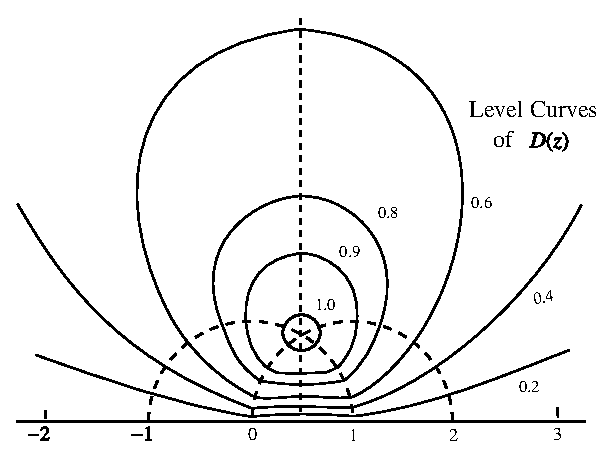
\includegraphics{figures/fig3.eps}
\end{figure}\pageoriginale

The above graph shows the behaviour of $D(z)$. (We have plotted the level curves $D(z)=0,.2,.4,.6,.8,.9,1.0$ in the upper half-plane. The values in the lower half-plane are obtained from $D(\overline{z})=-D(z)$. The maximum of $D$ is $1.0149\ldots$, attained at the point $(1+i\sqrt{3})/2$.)

The function $D(z)$, which was discovered by D. Wigner and S. Bloch (cf. \cite{art15-key1}), has many other beautiful properties. In particular :
\begin{itemize}
\item[(II)] $D(z)$, which is a real-valued function of $\mathbb{C}$, can be expressed in terms of a function of a single real variable, namely
\begin{equation}
D(z)=\frac{1}{2}\left[D\left(\dfrac{z}{\overline{z}}\right)+D\left(\dfrac{1-1/z}{1-1/\overline{z}}\right)+D\left(\dfrac{1/(1-z)}{1/(1-\overline{z})}\right)\right]\label{art15-eq2}
\end{equation}
which expresses $D(z)$ for arbitrary complex $z$ in terms of the function
$$
D(e^{i\theta})=\mathfrak{I}[\Li_{2}(e^{i\theta})]=\sum\limits^{\infty}_{n=1}\frac{\sin n\theta}{n^{2}}.
$$
Note\pageoriginale that the real part of $\Li_{2}$ on the unit circle is elementary :
$$
\sum\limits^{\infty}_{n=1}\frac{\cos n\theta}{n^{2}}=\frac{\pi^{2}}{6}-\frac{\theta(2\pi-\theta)}{4}\quad\text{for}\quad 0\leq \theta\leq 2\pi.)
$$
Formula (2) is due to Kummer.

\item[(III)] All of the functional equations satisfied by $\Li_{2}(z)$ lose the elementary correction terms (constants and products of logarithms) when expressed in terms of $D(z)$. In particular, one has the 6-fold symmetry
\begin{align}
D(z) &=D\left(1-\frac{1}{z}\right)=D\left(\dfrac{1}{1-z}\right)\notag\\
     &=-D\left(\dfrac{1}{z}\right)=-D(1-z)=-D\left(\dfrac{z}{z-1}\right)\label{art15-eq3}
\end{align}
and the five-term relation
\begin{equation}
D(x)+D(y)+D\left(\dfrac{1-x}{1-xy}\right)+D(1-xy)+D\left(\dfrac{1-y}{1-xy}\right)=0,\label{art15-eq4}
\end{equation}
while replacing $\Li_{2}$ by $D$ in the many-term relation \eqref{art15-eq1} makes the constant $C(f)$ disappear.
\end{itemize}

The functional equations become even cleaner if we think of $D$ as being a function not of a single complex number but of the cross-ratio of four such numbers, i.e. if we define
\begin{equation}
D(z_{0},z_{1},z_{2},z_{3})=D\left(\dfrac{z_{0}-z_{2}}{z_{0}-z_{3}}\dfrac{z_{1}-z_{3}}{z_{1}-z_{2}}\right)(z_{0},z_{1},z_{2},z_{3}\in \mathbb{C}).\label{art15-eq5}
\end{equation}

Then the symmetry properties \eqref{art15-eq3} say that $\widetilde{D}$ is invariant under even, anti-invariant under odd permutations of its four variables, the five-term relation \eqref{art15-eq4} takes on the attractive form
\begin{equation}
\sum\limits^{4}_{i=0}(-1)^{i}\widetilde{D}(z_{0},\ldots,\widehat{z}_{i},\ldots,z_{4})=0\quad (z_{0},\ldots,z_{4}\in \mathbb{P}^{1}(\mathbb{C})).\label{art15-eq6}
\end{equation}
(we will see the geometric interpretation of this later), and the multi-variable formula \eqref{art15-eq1} generalizes to the following beautiful formula :
$$
\sum\limits_{\substack{z_{1}\in f^{-1}(a_{1})\\ z_{2}\in f^{-1}(a_{2})\\ z_{3}\in f^{-1}(a_{3})}}\widehat{D}(z_{0},z_{1},z_{2},z_{3})=n\widetilde{D}(a_{0},a_{1},a_{2},a_{3})\quad (z_{0},a_{1},a_{2},a_{3}\in \mathbb{P}^{1})
$$\pageoriginale
where $f:\mathbb{P}^{1}\to \mathbb{P}^{1}$ is a function of degree $n$ and $a_{0}=f(z_{0})$. (Equation \eqref{art15-eq1} is the special case when $f$ is a polynomial, so $f^{-1}(\infty)$ is $\infty$ with multiplicity $n$.)

Finally, we mention that a real-analytic function on $\mathbb{P}^{1}(\mathbb{C})-\{0,1,\infty\}$ built up out of the polylogarithms in the same way as $D(z)$ was constructed from the dilogarithm, has been defined by Ramakrishnan \cite{art15-key6}. His function (slightly modified) is given by
$$
D_{m}(z)=\mathscr{R}\left(i^{m+1}\left[\sum\limits^{m}_{k=1}\frac{(-\log |z|)^{m-k}}{(m-k)!}\Li_{k}(z)-\frac{(\log |z|)^{m}}{2m!}\right]\right)
$$
(so $D_{1}(z)=\log |z^{1/2}-z^{-1/2}|, D_{2}(z)=D(z)$) and satisfies 
\begin{gather*}
D_{m}\left(\frac{1}{z}\right)=(-1)^{m-1}D_{m}(z),\\
\frac{\partial}{\partial z}D_{m}(z)=\frac{i}{2z}\left(D_{m-1}(z)+\frac{i}{2}\frac{(-i\log |z|)^{m-1}1+z}{(m-1)! \ 1-z}\right).
\end{gather*}
However, it does not seem to have analogues of the properties (II) and (III) : for example, it is apparently impossible to express $D_{3}(z)$ for arbitrary complex $z$ in terms of only the function $D_{3}(e^{i\theta})=\sum^{\infty}_{n=1}(\cos n\theta)/n^{3}$, and passing from $\Li_{3}$ to $D_{3}$ removes many but not all of the numerious lower-order terms in the various functional equations of the trilogarithm, e.g. :
\begin{align*}
& D_{3}(x)+D_{3}(1-x)+D_{3}\left(\dfrac{x}{x-1}\right)\\
&\quad =D_{3}(1)+\dfrac{1}{12}\log |x(1-x)|\log \left|\frac{x}{(1-x)^{2}}\right|\log \left|\frac{x^{2}}{1-x}\right|,\\
&\quad D_{3}\left(\dfrac{x(1-y)^{2}}{y(1-x)^{2}}\right)+D_{3}(xy)+D_{3}\left(\frac{x}{y}\right)-2D_{3}\left(\frac{x}{y}\frac{1-y}{1-x}\right)\\
&\quad {}-2D_{3}\left(\frac{x(1-y)}{x-1}\right)-2D_{3}\left(\frac{y(1-x)}{y-1}\right)-2D_{3}\left(\frac{1-y}{1-x}\right)\\
&\quad {}-2D_{3}(x)-2D_{3}(y)=2D_{3}(1)-\frac{1}{4}\log |xy|\log\left|\frac{x}{y}\right|\log \left|\frac{x}{y}\frac{(1-y)^{2}}{(1-x)^{2}}\right|.
\end{align*}\pageoriginale
Nevertheless, these higher Bloch-Wigner functions do occur. In studying the so-called ``Heegner points'' on modular curves, B. Gross and I had to study for $n=2,3,\ldots$ ``higher weight Green's functions'' for $\mathfrak{H}/\Gamma$ ($\mathfrak{H}=$ complex upper half-plane, $\Gamma=SL_{2}(\mathbb{Z})$ or a congruence subgroup). These are functions $G_{n}(z_{1},z_{2})=G^{\mathfrak{H}/\Gamma}_{n}(z_{1},z_{2})$ defined on $\mathfrak{H}/\Gamma\times \mathfrak{H}/\Gamma$, realanalytic in both variables except for a logarithmic singularity along the diagonal $z_{1}=z_{2}$, and satisfying $\Delta_{z_{1}}G_{n}=\Delta_{z_{2}}G_{n}=n(n-1)G_{n}$, where $\Delta_{z}=y^{2}(\partial^{2}/\partial x^{2}+\partial^{2}/\partial y^{2})$ is the hyperbolic Laplace operator with respect to $z=x+iy \in \mathfrak{H}$. They are obtained as
$$
G^{\mathfrak{G}/\Gamma}_{n}(z_{1},z_{2})=\sum\limits_{\gamma\in \Gamma}G^{\mathfrak{H}}_{n}(z_{1},\gamma z_{2})
$$
where $G^{\mathfrak{H}}_{n}$ is defined analogously to $G^{\mathfrak{G}/\Gamma}_{n}$ but with $\mathfrak{H}/\Gamma$ replaced by $\mathfrak{H}$. The functions $G^{\mathfrak{H}}_{n}(n=2,3,\ldots)$ are elementary, e.g.,
$$
G^{\mathfrak{H}}_{2}(z_{1},z_{2})=\left(1+\frac{|z_{1}-z_{2}|^{2}}{2y_{1}y_{2}}\right)\log \frac{|z_{1}-z_{2}|^{2}}{|z_{1}-\overline{z}_{2}|^{2}}+2.
$$
In between $G^{\mathfrak{H}}_{n}$ and $G^{\mathfrak{H}/\Gamma}_{n}$ are the functions $G^{\mathfrak{H}/\Gamma}_{n}=\Sigma_{r\in Z}G^{\mathfrak{H}}_{n}(z_{1},z_{2}+r)$. It turns out \cite{art15-key10} that these are expressible in terms of the $D_{m}(m=1,3,\ldots,2n-1)$, e.g.,
\begin{align*}
G^{\mathfrak{H}/Z}_{2}(z_{1},z_{2}) &= \frac{1}{4\pi^{2}y_{1}y_{2}}(D_{3}(e^{2\pi i(z_{1}-z_{2})})+D_{3}(e^{2\pi i(z_{1}-\overline{z}_{2})})\\
&\quad +\frac{y^{2}_{1}+y^{2}_{2}}{2y_{1}y_{2}}(D_{1}(e^{2\pi i(z_{1}-z_{2})})+D_{1}(e^{2\pi i(z_{1}-\overline{z}_{2})}))
\end{align*}
I do not know the reasons for this connection.

\section{Volumes of Hyperbolic 3-manifolds\ldots}\label{art15-sec4}\pageoriginale
The dilogarithm occurs in connection with measurement of volumes in Euclidean, spherical, and hyperbolic geometry. We will be concerned with the last of these. Let $\mathfrak{H}_{3}$ be the Lobachevsky space (space of non- Euclidean solid geometry). We will use the half-space model, in which $\mathfrak{H}_{3}$ is represented by $\mathbb{C}\times R_{+}$ with the standard hyperbolic metric in which the geodesics are either vertical lines or semicircles in vertical planes with endpoints in $\mathbb{C}\times \{0\}$ and the geodesic planes are either vertical planes or else hemispheres with boundary in $\mathbb{C}\times \{0\}$. {\em An ideal tetrahedron} is a tetrahedron whose vertices are all in $\partial \mathfrak{H}_{3}=\mathbb{C}\cup \{\infty\}=\mathbb{P}^{1}(\mathbb{C})$. Let $\Delta$ be such a tetrahedron. Although the vertices are at infinity, the (hyperbolic) volume is finite. It is given by
\begin{equation}
\Vol (\Delta)=\widehat{D}(z_{0},z_{1},z_{2},z_{3}),\label{art15-eq7}
\end{equation}
where $z_{0},\ldots,z_{3}\in\mathbb{C}$ are the vertices of $\Delta$ and $\widetilde{D}$ is the function defined in \eqref{art15-eq5}. In the special case that three of the vertices of $\Delta$ are $\infty$, $0$, and $1$, equation \eqref{art15-eq7} reduces to the formula (due essentially to Lobachevsky)
\begin{equation}
\Vol (\Delta)=D(z).\label{art15-eq8}
\end{equation}
\begin{figure}[H]
\centering
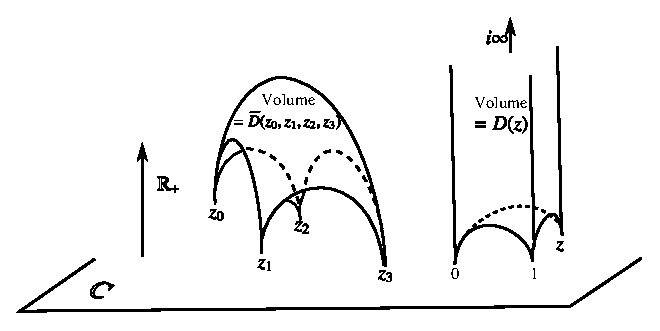
\includegraphics{figures/fig4.eps}
\end{figure}

In fact, equations \eqref{art15-eq7} and \eqref{art15-eq8} are equivalent since any 4-tuple of points $z_{0},\ldots,z_{3}$ can be brought into the form $\{\infty,0,1,z\}$ by the action of some element of $SL_{2}(\mathbb{C})$ on $\mathbb{P}^{1}(\mathbb{C})$, and the group $SL_{2}(\mathbb{C})$ acts on $\mathfrak{H}_{3}$ by isometries.

The\pageoriginale (anti-) symmetry properties of $\widetilde{D}$ under permutations of the $z_{i}$ are obvious from the geometric interpretation \eqref{art15-eq7}, since renumbering the vertices leaves $\Delta$ unchanged but may reverse its orientation. Formula \eqref{art15-eq6} is also an immediate consequence of \eqref{art15-eq7}, since the five tetrahedra spanned by four at a time of $z_{0},\ldots,z_{4}\in \mathbb{P}^{1}(\mathbb{C})$, counted positively or negatively as in \eqref{art15-eq6}, add up algebraically to the zero 3-cycle.

The reason that we are interested in hyperbolic tetrahedra is that these are the building blocks of hyperbolic 3-manifolds, which in turn (according to Thurston) are the key objects for understanding three-dimensional geometry and topology. A hyperbolic 3-manifold is a 3-dimensional riemannian manifold $M$ which is locally modelled on (i.e., isometric to portions of) hyperbolic 3-space $\mathfrak{H}_{3}$; equivalently, it has constant negative curvature $-1$. We are interested in complete oriented hyperbolic 3-manifolds which have finite volume (they are then either compact or have finitely many ``cusps'' diffeomorphic to $S^{1}\times S^{1}\times \mathbb{R}_{+}$). Such a manifold can obviously be triangulated into small geodesic simplices which will be hyperbolic tetrahedra. Less obvious is that (possibly after removing from $M$ a finite number of closed geodesics) there is always a triangulation into {\em ideal} tetrahedra (the part of such a tetrahedron going out towards a vertex at infinity will then either tend to a cusp of $M$ or else spiral in around one of the deleted curves). Let these tetrahedra be numbered $\Delta_{1},\ldots,\Delta_{n}$ and assume (after an isometry of $\mathfrak{H}_{3}$ if necessary) that the vertices of $\Delta_{v}$ are at $\infty$, $0$, $1$ and $z_{v}$. Then
\begin{equation}
\Vol (M)=\sum\limits^{n}_{v=1}D(z_{v}).\label{art15-eq9}
\end{equation}
Of course, the numbers $z_{v}$ are not uniquely determined by $\Delta_{v}$ since they depend on the order in which the vertices were sent to $\{\infty,0,1,z_{v}\}$, but the non-uniqueness consists (since everything is oriented) only in replacing $z_{v}$ by $1-1/z_{v}$ or $1/(1-z_{v})$ and hence does not affect the value of $D(z_{v})$.

One of the objects of interest in the study of hyperbolic 3-manifolds is the ``volume spectrum''
$$
\mathbf{Vol}=\{\Vol(M)|M\text{~ hyperbolic 3-manifold}\}\subset \mathbb{R}_{+}.
$$
From the work of J{\o}rgensen and Thurston one knows the {\bf Vol} is a countable and well-ordered subset of $\mathbb{R}_{+}$ (i.e. every subset has a smallest element), and its exact nature is of considerable interest both in topology and number theory. Equation \eqref{art15-eq9} as it stands says nothing about this set since\pageoriginale any real number can be written as a finite sum of values $D(z)$, $z\in \mathbb{C}$. However, the parameters $z_{v}$ of the tetrahedra triangulating a complete hyperbolic 3-manifold satisfy an extra relation, namely
\begin{equation}
\sum\limits^{n}_{v=1}z_{v}\wedge (1-z_{v})=0,\label{art15-eq10}
\end{equation}
where the sum is taken in the abelian group $\wedge^{2}\mathbb{C}^{\times}$ (the set of all formal linear combinations $x\wedge y$, $x$, $y\in \mathbb{C}^{\times}$, subject to the relations $x\wedge x=0$ and $(x_{1}x_{2})\wedge y=x_{1}\wedge y+x_{2}\wedge y$). (This follows from assertions in \cite{art15-key3} or form Corollary 2.4 of \cite{art15-key5} applied to suitable $x$ and $y$). Now \eqref{art15-eq9} {\em does} give information about {\bf Vol} because the set of numbers $\Sigma^{n}_{v=1}D(z_{v})$ with $z_{v}$ satisfying \eqref{art15-eq10} is countable. This fact was proved by Bloch \cite{art15-key1}. To make a more precise statement, we introduce the {\em Bloch group}. Consider the abelian group of formal sums $[z_{1}]+\cdots+[z_{n}]$ with $z_{1},\ldots,z_{n}\in \mathbb{C}^{\times}-\{1\}$ satisfying \eqref{art15-eq10}. As one easily checks, it contains the elements
\begin{equation}
[x]+\left[\frac{1}{x}\right], \ [x]+[1-x], \ [x]+[y]+\left[\frac{1-x}{1-xy}\right]+[1-xy]+\left[\frac{1-y}{1-xy}\right]\label{art15-eq11}
\end{equation}
for all $x$ and $y$ in $\mathbb{C}^{\times}-\{1\}$ with $xy\neq 1$, corresponding to the symmetry properties and 5-term relation satisfied by $D(\cdot)$. The Block group is defined as
\begin{equation}
\begin{array}{p{10cm}}
$\mathscr{B}_{\mathbb{C}}=\{[z_{1}]+\cdots+[z_{n}]$ satisfying \eqref{art15-eq10}\}/(subgroup generated by the elements \eqref{art15-eq11})
\end{array}\label{art15-eq12}
\end{equation}
(this is slightly different from the usual definitions). The definition of the Block group in terms of the relations satisfied by $D(\cdot)$ makes it obvious that $D$ extends to a linear map $D:\mathscr{B}_{\mathbb{C}}+\mathbb{R}$ by $[z_{1}]+\cdots+[z_{n}]\mapsto D(z_{1})+\cdots+D(z_{n})$, and Bloch's result (related to Mostow rigidity) says that the set $D(\mathscr{B}_{\mathbb{C}})$ coincides with $D(\mathscr{B}_{\overline{\mathbb{Q}}})$ (where $\mathscr{B}_{\overline{\mathbb{Q}}}$ is defined by \eqref{art15-eq12} but with the $z_{v}$ lying in $\overline{\mathbb{Q}}^{\times}-\{1\}$). Thus $D(\mathscr{B}_{\mathbb{C}})$ is countable, and \eqref{art15-eq9} and \eqref{art15-eq10} imply that {\bf Vol} is contained in this countable set. The structure of $\mathscr{B}_{\overline{\mathbb{Q}}}$ which is very subtle, will be discussed below.

We give an example of a non-trivial element of the Bloch group. For convenience, set $\alpha=\dfrac{1-\sqrt{-7}}{2}$, $\beta=\dfrac{-1-\sqrt{-7}}{2}$. Then 
\begin{align*}
& 2\left(\dfrac{1+\sqrt{-7}}{2}\right)\wedge \left(\frac{1-\sqrt{-7}}{2}\right)+\left(\dfrac{-1+\sqrt{-7}}{4}\right)\wedge\left(\frac{5-\sqrt{-7}}{4}\right)\\
& 2(-\beta)\wedge\alpha+\left(\frac{1}{\beta}\right)\wedge\left(\frac{\alpha^{2}}{\beta}\right)=\beta^{2}\wedge \alpha-\beta\wedge\alpha^{2}=2\cdot \beta\wedge \alpha-2-\cdot \beta \wedge\alpha=0,
\end{align*}\pageoriginale
so
\begin{equation}
2\left[\dfrac{1+\sqrt{-7}}{2}\right]+\left[\dfrac{-1+\sqrt{-7}}{4}\right]\in \mathscr{B}_{\mathbb{C}}.\label{art15-eq13}
\end{equation}
This example should make it clear why non-trivial elements of $\mathscr{B}_{\mathbb{C}}$ can only arise from algebraic numbers --- the key relations $1+\beta=\alpha$ and $1-\beta^{-1}=\alpha^{2}/\beta$ above forced $\alpha$ and $\beta$ to be algebraic.

\section{\ldots and values of Dedekind zeta functions}\label{art15-sec5}
Let $F$ be an algebraic number field, say of degree $N$ over $\mathbb{O}$. Among its most important invariants are the discriminant $d$, the numbers $r_{1}$ and $r_{2}$ of real and imaginary archimedean valuations, and the Dedekind zeta-function $\zeta_{F}(s)$. For the non-number-theorist we recall the (approximate) definitions. The field $F$ can be represented as $\mathbb{Q}(\alpha)$ where $\alpha$ is a root of an irreducible monic polynomial $f\in \mathbb{Z}[x]$ of degree $N$. The discriminant of $f$ is an integer $d_{f}$ and $d$ is given by $c^{-2}d_{f}$ for some natural number $c$ with $c^{2}|d_{f}$. The polynomial $f$, which is irreducible over $\mathbb{Q}$, in general becomes reducible over $\mathbb{R}$, where it splits into $r_{1}$ linear and $r_{2}$ quadratic factors (thus $r_{1}\geq 0$, $r_{2}\geq 0$, $r_{1}+2r_{2}=N$). It also in general becomes reducible when it is reduced modulo a prime $p$, but if $p\nmid d_{f}$ then its irreducible factors modulo $p$ are all distinct, say $r_{1,p}$ linear factors, $r_{2,p}$ quadratic ones, etc. (so $r_{1,p}+2r_{2,p}+\cdots =N$). Then $\zeta_{F}(s)$ is the Dirichlet series given by an Euler product $\Pi_{p}Z_{p}(p^{-s})^{-1}$ where $Z_{p}(t)$ for $p\nmid d_{f}$ is the monic polynomial $(1-t)^{r_{1,p}}(1-t^{2})^{r_{2,p}}\ldots$ of degree $N$ and $Z_{P}(t)$ for $p|d_{f}$ is a certain monic polynomial of degree $\leq N$. Thus $(r_{1},r_{2})$ and $\zeta_{F}(s)$ encode the information about the behaviour of $f$ (and hence $F$) over the real and $p$-adic numbers, respectively.

As an example, let $F$ be an imaginary quadratic field $\mathbb{O}(\sqrt{-a})$ with $a\geq 1$ squarefree. Here $N=2$, $d=-a$ or $-4a$, $r_{1}=0$, $r_{2}=1$. The Dedekind zeta function has the form $\sum\limits_{n\geq 1}r(n)n^{-s}$ where $r(n)$ counts representations of $n$ by certain quadratic forms of discriminant $d$; it can also be represented as the product of the Riemann zeta function $\zeta(s)=\zeta^{(s)}_{\mathbb{O}}$\pageoriginale with an $L$-series $L(s)=\sum\limits_{n\geq 1}\left(\frac{d}{n}\right)n^{-s}$ where $\left(\frac{d}{n}\right)$ is a symbol taking the values $\pm 1$ or $0$ and which is periodic of period $|d|$ in $n$. Thus for $a=7$
\begin{align*}
\zeta_{\mathbb{Q}(\sqrt{-7})}(s) &= \frac{1}{2}\sum\limits_{(x,y)\neq (0,0)}\frac{1}{(x^{2}+xy+2y^{2})^{s}}\\
&= \left(\sum\limits^{\infty}_{n=1}n^{-s}\right)\left(\sum\limits^{\infty}_{n=1}\left(\frac{-7}{n}\right)n^{-s}\right)
\end{align*}
where $\left(\frac{-7}{n}\right)$ is $+1$ for $n\equiv 1$, $2$, $4(\mod 7)$, $-1$ for $n\equiv 3,5,6(\mod 7)$, and $0$ for $n\equiv 0(\mod 7)$.

One of the questions of interest is the evaluation of the Dedekind zeta function at suitable integer arguments. For the Riemann zeta function we have the special values cited at the beginning of this paper. More generally, if $F$ is totally real (i.e., $r_{1}=N$, $r_{2}=0$), then a theorem of Siegel and Klingen implies that $\zeta_{F}(m)$ for $m=2,4,\ldots$ equals $\pi^{mN}/\sqrt{d}$ times a rational number. If $r_{2}>0$, then no such simple result holds. However, in the case $F=\mathbb{Q}(\sqrt{-a})$, then using the representation $\zeta_{F}(s)=\zeta(s)L(s)$ and the formula $\zeta(2)=\pi^{2}/6$ and writing the periodic function $(d/n)$ as a finite linear combination of terms $e^{2\pi in \ \ d}$, we obtain
$$
\zeta_{F}(2)=\frac{\pi^{2}}{6\sqrt{|d|}}\sum\limits^{|d|-1}_{n=1}\left(\dfrac{d}{n}\right)D(e^{2\pi in \ \ d})\quad (F\text{~ imaginary quadratic}),
$$
e.g.,
$$
\zeta_{\mathbb{Q}(\sqrt{-7})}(2)=\frac{\pi^{2}}{3\sqrt{7}}\left(D(e^{2\pi i/7})+D(e^{4\pi i/7})-D(e^{6\pi i/7})\right)
$$
Thus the values of $\zeta_{F}(2)$ for imaginary quadratic fields can be expressed in closed form in terms of values of the Bloch-Wigner function $D(z)$ at algebraic arguments $z$.

By using the ideas of the last section we can prove a much stronger statement. Let $\mathscr{O}$ denote the ring of integers of $F$ (this is the $\mathbb{Z}$-lattice in $\mathbb{C}$ spanned by $1$ and $\sqrt{-a}$ or $(1+\sqrt{-a})/2$, depending whether $d=-4a$ or $d=-a$). Then the group $\Gamma=SL_{2}(\mathscr{O})$ is a discrete subgroup of $SL_{2}(\mathbb{C})$ and therefore acts on hyperbolic space $\mathfrak{H}_{3}$ by isometries. A classical result of Humbert gives the volume of the quotient space $\mathfrak{H}_{3}/\Gamma$ as $|d|^{3/2}\times \zeta_{F}(2)/4\pi^{2}$.\pageoriginale On the other hand, $\mathfrak{H}_{3}/\Gamma$ (or, more precisely, a certain covering of it of low degree) can be triangulated into ideal tetrahedra with vertices belonging to $\mathbb{P}^{1}(F)\subset \mathbb{P}^{1}(C)$, and this leads to a representation
$$
\zeta_{F}(2)=\frac{\pi^{2}}{3|d|^{3/2}}\sum\limits_{v}n_{v}D(z_{v})
$$
with $n_{v}$ in $\mathbb{Z}$ and $z_{v}$ {\em in $F$ itself} rather than in the much larger field $\mathbb{Q}(e^{2\pi i \ \ d})$(\cite{art15-key8}, Theorem 3). For instance, in our example $F=\mathbb{Q}(\sqrt{-7})$ we find
$$
\zeta_{F}(2)=\frac{4\pi^{2}}{21\sqrt{7}}\left(2D\left(\frac{1+\sqrt{-7}}{2}\right)+D\left(\frac{-1+\sqrt{-7}}{4}\right)\right).
$$
This equation together with the fact that $\zeta_{F}(2)=1.89484144897\ldots\neq 0$ implies that the element \eqref{art15-eq13} has infinite order in $\mathscr{B}_{\mathbb{C}}$.

In \cite{art15-key8}, it was pointed out that the same kind of argument works for all number fields, not just imaginary quadratic ones. If $r_{2}=1$ but $N>2$ then one can again associate to $F$ (in many different ways) a discrete subgroup $\Gamma\subset SL_{2}(\mathbb{C})$ such that $\Vol(\mathfrak{H}_{3}/\Gamma)$ is a rational multiple of $d|^{1/2}\zeta_{F}(2)\times \pi^{2(1-N)}$. This manifold $\mathfrak{H}_{3}/\Gamma$ is now compact, so the decomposition into ideal tetrahedra is a little less obvious than in the case of imaginary quadratic $F$, but by decomposing into non-ideal tetrahedra (tetrahedra with vertices in the interior of $\mathfrak{H}_{3}$) and writing these as differences of ideal ones, it was shown that the volume is an integral linear combination of values of $D(z)$ with $z$ of degree at most $4$ over $F$. For $F$ completely arbitrary there is still a similar statement, except that now one gets discrete groups $\Gamma$ acting on $\mathfrak{H}^{r_{2}}_{3}$; the final result (\cite{art15-key8}, Theorem 1) is that $|d|^{1/2}\times \zeta_{F}(2)/\pi^{2(r_{1}+r_{2})}$ is a rational linear combination of $r_{2}$-fold products $D(z^{(1)})\ldots D(z^{(r_{2})})$ with each $z^{(i)}$ of degree $\leq 4$ over $F$ (more precisely, over the $i^{\text{th}}$ complex embedding $F^{(i)}$ of $F$, i.e. over the subfield $\mathbb{Q}(\alpha^{(i)})$ of $\mathbb{C}$ where $\alpha^{(i)}$ is one of the two roots of the $i^{\text{th}}$ quadratic factor of $f(x)$ over $\mathbb{R}$).

But in fact much more is true : the $z^{(i)}$ can be chosen in $F^{(i)}$ itself (rather than of degree $4$ over this field), and the phrase ``rational linear combination of $r_{2}$-fold products'' can be replaced by ``rational multiple of an $r_{2}\times r_{2}$ determinant.'' We will not attempt to give more than a very sketchy account of why this is true, lumping together work of Wigner, Bloch, Dupont, Sah, Levine, Merkuriev, Suslin, \ldots for the purpose (references are \cite{art15-key1}, \cite{art15-key3}, and the survey paper \cite{art15-key7}). This work connects the Bloch\pageoriginale group defined in the last section with the algebraic $K$-theory of the underlying field; specifically, the group\footnote[1]{It should be mentioned that the definition of $\mathscr{B}_{F}$ which we gave for $F=\mathbb{C}$ or $\overline{\mathbb{Q}}$ must be modified slightly when $F$ is a number field because $F^{\times}$ is no longer divisible; however, this is a minor point, affecting only the torsion in the Bloch group, and will be ignored here.} $\mathscr{B}_{F}$ is equal, at least after tensoring it with $\mathbb{O}$, to a certain quotient $K^{\text{ind}}_{3}(F)$ of $K_{3}(F)$. The exact definition of $K^{\text{ind}}_{3}(F)$ is not relevant here. What is relevant is that this group has been studied by Borel \cite{art15-key2}, who showed that it is isomorphic (modulo torsion) to $\mathbb{Z}^{r_{2}}$ and that there is a canonical homomorphism, the ``regulator mapping,'' from it into $\mathbb{R}^{r_{2}}$ such that the co-volume of the image in a non-zero rational multiple of $|d|^{a/2}\zeta_{F}(2)/\pi^{2r_{1}+2r_{2}}$; moreover, it is known that under the identification of $K^{\text{ind}}_{3}(F)$ with $\mathscr{B}_{F}$ this mapping corresponds to the composition $\mathscr{B}_{F}\to (\mathscr{B}_{\mathbb{C}})^{r_{2}}\xrightarrow{D}\mathbb{R}^{r_{2}}$, where the first arrow comes from using the $r_{2}$ embeddings $F\subset \mathbb{C}(\alpha\to \alpha^{(i)})$. Putting all this together gives the following beautiful picture : The group $\mathscr{B}_{F}/\{\text{torsion}\}$, is isomorphic to $\mathbb{Z}^{r_{2}}$. Let $\zeta_{1},\ldots,\zeta_{r_{2}}$ by any $r_{2}$ linearly independent elements of it, and form the matrix with entires $D(\zeta^{(i)}_{j})$, $(i,j=1,\ldots,r_{2})$. Then the determinant of this matrix is a non-zero rational multiple of $|d|^{1/2}\zeta_{F}(2)/\pi^{2r_{1}+2r_{2}}$. If instead of taking any $r_{2}$ linearly independent elements we choose the $\zeta_{j}$ to be a basis of $\mathscr{B}_{F}/\{\text{torsion}\}$, then this rational multiple (chosen positively) is an invariant of $F$, independent of the choice of $\zeta_{j}$. This rational multiple is then conjecturally related to the quotient of the order of $K_{3}(F)_{\text{torsion}}$ by the order of the finite group $K_{2}(\mathscr{O}_{F})$ where $\mathscr{O}_{F}$ denotes the ring of integers of $F$ (Lichtenbaum conjectures).

This all sounds very abstract, but it is fact not. There is a reasonably efficient algorithm to produce many elements of $\mathscr{B}_{F}$ for any number field $F$. If we do this, for instance, for $F$ an imaginary quadratic field, and compute $D(\zeta)$ for each element $\zeta\in \mathscr{B}_{F}$ which we find, then after a while we are at least morally certain of having identified the lattice $D(\mathscr{B}_{F})\subset \mathbb{R}$ exactly (after finding $k$ elements at random, we have only about one chance in $2^{k}$ of having landed in the same non-trivial sublattice each time). By the results just quoted, this lattice is generated by a number of the form $\kappa |d|^{3/2}\zeta_{F}(2)/\pi^{2}$ with $\kappa$ rational, and the conjecture referred to above says that $\kappa$ should have the form $\frac{3}{2T}$ where $T$ is the order of the finite group $K_{2}(\mathscr{O}_{F})$, at least for $d<-4$ (in this case the order of $K_{3}(F)_{\text{torsion}}$ is always 24). Calculations done by H. Gangl in Bonn for several hundred imaginary quadratic fields support this; the $\kappa$ he found all have the form $\frac{3}{2T}$\pageoriginale for some integer $T$ and this integer agrees with the order of $K_{2}(\mathscr{O}_{F})$ in the few cases where the latter is known. Here is a small excerpt from his tables :
\begin{center}
\tabcolsep=1.7pt
\begin{tabular}{@{}c|ccccccccccccccccccc@{}}
$|d|$ & 7 & 8 & 11 & 15 & 19 & 20 & 23 & 24 & 31 & 35 & 39 & 40 & \ldots & 303 & 472 & 479 & 491 & 555 & 583\\
\hline
$T$ & 2 & 1 & 1 & 2 & 1 & 1 & 2 & 1 & 2 & 2 & 6 & 1 & \ldots & 22 & 5 & 14 & 13 & 28 & 34
\end{tabular}
\end{center}
(the omitted values contain only the primes 2 and 3; 3 occurs whenever $d\equiv 3(\mod 9)$ and there is also some regularity in the powers of 2 occurring). Thus one of the many virtues of the mysterious dilogarithm is that it gives, at least conjecturally, an effective way of calculating the orders of certain groups in algebraic $K$-theory!

To conclude, we mention that Borel's work connects not only $K^{\text{ind}}_{3}(F)$ and $\zeta_{F}(2)$ but more generally $K^{\text{ind}}_{2m-1}(F)$ and $\zeta_{F}(m)$ for any integer $m>1$. No elementary description of the higher $K$-groups analogous to the description of $K_{3}$ in terms of $B$ is known, but one can at least speculate that these groups and their regulator mappings may be related to the higher polylogarithms and that, more specifically, the value of $\zeta_{F}(m)$ is always a simple multiple of a determinant ($r_{2}\times r_{2}$ or $(r_{1}+r_{2})\times (r_{1}+r_{2})$ depending whether $m$ is even or odd) whose entries are linear combinations of values of the Bloch-Wigner-Ramakrishnan function $D_{m}(z)$ with arguments $z\in F$. As the simplest case, one can guess that for a {\em real} quadratic field $F$ the value of $\zeta_{F}(3)/\zeta(3)=L(3)$, where $L(s)$ is a Dirichlet $L$-Function of a real quadratic character of period $d$) is equal to $d^{-5/2}$ times a simple rational linear combination of differences $D_{3}(x)-D_{3}(x')$ with $x\in F$, where $x'$ denotes the conjugate of $x$ over $\mathbb{Q}$. Here is one (numerical) example of this :
\begin{align*}
2^{-5}5^{5/2}\zeta_{\mathbb{Q}(\sqrt{5})}(3)/\zeta(3) &= D_{3}\left(\frac{1+\sqrt{5}}{2}\right)-D_{3}\left(\frac{1-\sqrt{5}}{2}\right)-{}\\
&\quad {}-\frac{1}{3}[D_{3}(2+\sqrt{5})-D_{3}(2-\sqrt{5})]
\end{align*}
(both sides are equal approximately to $1.493317411778544726$). I have found many other examples, but the general picture is not yet clear.

\begin{thebibliography}{99}
\bibitem{art15-key1} \textsc{S. Bloch :}\pageoriginale Applications of the dilogarithm function in algebraic $K$-theory and algebraic geometry, in : {\em Proc. of the International Symp. on Alg . Geometry,} Kinokuniya, Tokyo, 1978.

\bibitem{art15-key2} \textsc{A. Borel :} Commensurability classes and volumes of hyperbolic 3-manifolds, {\em Ann. Sc. Norm. Sup. Pisa,} 8 (1981) pp. 1-33.

\bibitem{art15-key3} \textsc{J. L. Dupont} and \textsc{C. H. Sah :} Scissors congruences II, {\em J. Pure and Applied Algebra}, 25 (1982), 159-195.

\bibitem{art15-key4} \textsc{L. Lewin :} {\em Polylogarithms and associated functions} (title of original 1958 edition : {\em Dilogarithms and associated functions}). North Holland, New York, 1981.

\bibitem{art15-key5} \textsc{W. Neumann} and \textsc{D. Zagier :} Volumes of hyperbolic 3-manifolds, {\em Topology,} 24 (1985), 307-332.

\bibitem{art15-key6} \textsc{D. Ramakrishnan :} Analogs of the Bloch-Wigner function for higher polylogarithms, {\em Contemp. Math.,} 55 (1986), 371-376.

\bibitem{art15-key7} \textsc{A. A. Suslin :} Algebraic $K$-theory of fileds, in : {\em Proceedings of the ICM Berkeley} 1986 A.M.S. (1987), 222-244.

\bibitem{art15-key8} \textsc{D. Zagier :} Hyperbolic manifolds and special values of Dedekind zeta-functions, {\em Invent. Math.,} 83 (1986), 285-301.

\bibitem{art15-key9} \textsc{D. Zagier :} On an approximate identity of Ramanujan, {\em Proc. Ind. Acad. Sci.} ({\em Ramanujan Centenary Volume}) 97 (1987), 313-324.

\bibitem{art15-key10} \textsc{D. Zagier :} Green's functions of quotients of the upper half-plane (in preparation.)
\end{thebibliography}

\bigskip
\noindent
{\small Max-Planck-Institut f\"ur Mathematik},

\noindent
{\small Gottfried-Claren-Stra{\ss}e 26, D-5300 Bonn, FRG.

\medskip
\noindent
{\small and}
\medskip

\noindent
{\small Department of Mathematics},

\noindent
{\small University of Maryland,}

\noindent
{\small College Park, Maryland 20742, USA.}




